\chapter{Details of the Monte Carlo Code}\label{chp:chp2}

%\begin{flushright}
%  {\em QUOTE GOES HERE }\\
%
%\ \
%
%\normalsize
%{AUTHOR}  
%\end{flushright}


\section{Monte Carlo Methods}
	 
	 \noindent{The name 'Monte Carlo' describes a class of modelling techniques that employ a stochastic approach to simulating mathematical and physical situations that are otherwise difficult or impossible to solve.  By repeatedly sampling random numbers from a probability distribution, numerical results to non-analytic problems may be obtained.  The approach was first used by researchers at Los Alamos in the late 1940s who adopted the method to model the transport of neutrons.  It is from the code name for this project, 'Monte Carlo', that the methods derive their name.  }
	 
	 As the available computing power increased over the following decades, Monte Carlo methods became more and more useful as a means of solving complex problems and are now used widely across numerous fields including mathematics, statistics, engineering, finance, the physical sciences and many others.  The nature of the approach means that they are particularly well-suited to problems with multiple degrees of freedom, and especially when any of these degrees are coupled.  By using random numbers to represent quantities that parametrize a physical problem, a model may be generated that simulates a solution to the problem using a pseudo-random number generator.   It must be the case that the quantities that characterize the problem may be represented by a continuous distribution in the range [0,1] in order that randomly generated numbers may be translated into physical properties.  
	 
	 For each randomly-generated input, the model of interest is applied and an output - a 'possible outcome' - is obtained.  By iterating this process many times with randomly-generated inputs each time, many possible outcomes are generated and a probability distribution may be built up.  The interpretation of the outputted probability distribution is dependent on the manner of utilisation of the Monte Carlo method.  For example, the iterative procedure may be used to determine best-fitting parameters of a model or may be used to find the mean-free path of a photon.  In the former case, the multi-dimensional probability distribution may be analysed to determine the most representative model or models whereas in the latter case the probability distribution is equivalent to an energy distribution.
	 
	 Clearly, Monte Carlo simulations are limited by their finite nature and will never produce a perfect solution.  However, this does not mean that Monte Carlo simulations are lacking in rigour.  It may be shown that the error in a Monte Carlo model is approximately $\sim \frac{1}{\sqrt{n}}$ for large $n$, where $n$ is the number of quanta used in the simulation.  The error may therefore be made as small as required by increasing the number of quanta used in the simulation subject to the restrictions of computing time and expense.
	 
	 In the next section, I discuss the use of Monte Carlo methods as applied to radiative transfer problems and  specifically to DAMOCLES.  I discuss the computational aspects of my work and the architecture of the code in section \ref{damocles_struct} before finally discussing the limitations of the code and its potential for future developments in section \ref{limitations}.
	 
\section{Radiative Transfer and the Monte Carlo Method}
\label{rt}

 The application of Monte Carlo codes to radiative transfer problems in astrophysics has a strong history.  Numerous codes that utilise this stochastic methodology have been written in the past few decades in order to model the transport of photon packets through various media.  The energy to be transported throughout the region of interest is discretised into packets and the path of each packet is calculated according to the properties of the environments that it passes through during its lifetime.  Collating the escaped packets at the end of the simulation produces an energy distribution. 

There exist several Monte Carlo radiative transfer codes that use this technique in order to model the transfer of line emission through a nebula to produce a synthetic spectrum. There also exist a number of codes that treat the continuous emission and absorption of energy in dusty environments in order to produce and fit a spectral energy distribution (SED).  Models of supernovae have been produced using both approaches and well-fitting spectra and SEDs have been generated but never, according to the best of my knowledge, has the mechanism been employed to produce sophisticated models of line profiles in expanding dusty regions.  In this new code, we seek to apply the technique to an expanding dusty medium in order to consider the effects on a single emitted line profile.

Previous work by Leon Lucy has considered the problem of dust-induced asymmetric line profiles in the ejecta of supernovae and he has published results derived both analytically and using simple Monte Carlo simulations.  These simulations appear to be the only published instances of a numerical approach to studying this spectral feature.  The DAMOCLES code adopts the same technique as the original modelling by Leon Lucy but allows for a considerably more complex treatment of the composition, geometry and motion of the dusty medium.

Radiative transfer methods as applied to supernovae generally treat a wide wavelength range and seek to conserve the total energy.  In the case of SED modelling, this is often achieved by dividing the total energy into packets of equal weight and energy, and iteratively determining the temperature and ionization structure.  In this work, the approach we adopt is somewhat simpler as only a very narrow wavelength range need be considered.  Rather than seeking to conserve the total energy, we assume that any packet absorbed by dust would be re-emitted outside the wavelength range of interest and thus no longer contributes to the resulting line profile.  Any absorbed packet is therefore removed from circulation.  In addition to this, the absorption and scattering of radiation by dust is independent of temperature and there is therefore no need to calculate temperatures throughout the nebula.  Similarly, in the case of radiative modelling of synthetic spectra of the ejecta of supernovae, approximations such as the Sobolev approximation are often employed to handle the blending of lines more efficiently.  This is unnecessary here as only a single line or doublet is ever treated and a comparatively narrow wavelength range considered. 

The subtleties of the problem we consider here lie in the treatment of an atmosphere expanding as fast as 10\% of the speed of light.  Lorentz transforms must be carefully applied in order that packets experience the appropriate degree of frequency shifting at emission and at each subsequent scattering event.  In this respect, the code is analogous to Monte Carlo radiative transfer models of electron scattering published by \ref{}.  Indeed, similar features are observed in the outputs of both.

Throughout this section, I will describe the principles, assumptions and techniques adopted in the production of the DAMOCLES before I move on to address the mechanics and architecture of the code itself.  DAMOCLES stands for \textbf{D}ust-\textbf{A}ffected \textbf{M}odels \textbf{O}f \textbf{C}haracteristic \textbf{L}ine \textbf{E}mission in \textbf{S}upernovae.
 

	\subsection{Energy Packets}
	
	The fundamental principle underlying the transport of radiation throughout a dusty nebula is that the radiation be discretised into packets.  Each of these packets is then propagated throughout the nebula and ultimately contributes a fraction of the final energy distribution.  At the start of the simulation, each packet is assumed to consist of $n$ photons of frequency $\nu_0$, the rest frequency of the line to be modelled.  All packets therefore begin life with initial energy

\begin{equation}
	E_0=nh\nu_0
\end{equation}
	
	
	where $h$ is Planck's constant.  As the packets move through the ejecta, they are scattered off high-velocity dust grains and after each scattering event, the frequency of the packet is altered.  In Monte Carlo simulations that model non-moving atmospheres, packets are usually taken to be of constant energy.  When the frequency of a packet is altered after an event, the energy of that packet is kept constant and the number of real photons contained within it assumed to change.  However, in the case of dust scattering, the number of real photons is conserved and thus the energy of the packet is altered.  This is most easily achieved by weighting each packet over all scattering events as 
	
\begin{equation}
	w=\prod_{scat} \frac{\nu'}{\nu}
\end{equation}

\noindent where $w$ is the weight of the packet.  The final energy of each packet is then $E =w E_0$, where $E_0$ is the initial energy of the packet.  The final dust-affected line profile is compiled by adding the total energy of all packets in a specific frequency bin in order to produce a histogram.
	
	In these models, unlike fully self-consistent SED radiative transfer models, there is no requirement that the total energy be conserved.  We drop this traditional requirement since radiation that is absorbed by dust is re-emitted outside of the wavelength range of interest and thus no longer contributes any flux to the resulting line profile.  Packets that are absorbed may be safely removed from the simulation.
	
	\subsection{Initialisation and the Grid}
	
	The supernova ejecta is approximated by a three-dimensional cartesian grid, each cell of which is assumed to have uniform density and composition.  By default, the ejecta occupies a shell between inner radius $R_{in}$ and outer radius $R_{out}$. The grid extends from $-R_{out}$ to $+R_{out}$ in each of the three axes.  Each side is split into the same number of divisions and thus each cell is a cube of volume $R_{out}^3/n_{div}^3$ where $n_{div}$ is the number of divisions along each axis and is specified by the user.  For the remainder of this thesis, a spherically symmetric situation is assumed and in all modelling and testing the grid is constructed in this manner.  However, there are no assumptions of symmetry in the code and a cartesian grid was adopted in order to allow for arbitrary geometries to be modelled in the future e.g. ellipsoidal or toroidal ejecta distributions.
	
	  Both gas and dust are by default assumed to have a power-law distribution declared as  $\rho(r) \propto r^{-\beta}$ between $R_{in}$ and $R_{out}$.  The distribution of gas determines the emissivity distribution and thus the starting positions of the packets in the simulation (see section \ref{sctn:em_prop}).  However, after the initial emission of energy packets, the gas plays no further role in the simulation as only interactions with dust grains are of interest here.  By default, the dust is coupled to the gas and thus follows the same smooth power-law distribution previously described with exponent $-\beta$.  The dust density in each cell is therefore calculated as
	
\begin{equation}
\rho (r)= \frac{M_{tot}(3-\beta)}{4\pi (R_{out}^{3-\beta}-R_{in}^{3-\beta})}
\end{equation}
	
	
\noindent where $r$ is the radial distance from the centre of the cell to the origin and $M_{tot}$ is the total desired dust mass to model.  Any cell whose centre falls outside of the bounds of the supernova ejecta has dust density set to zero.  If the dust and gas are decoupled then the user must specify distinct profiles for the gas and the dust; that is, separate power laws must be declared and independent inner and outer radii specified.  This allows for more sophisticated modelling of, for example, circumstellar shells or dense cores of dust formation surrounded by more diffuse gas.

It is known from SED modelling that clumped environments produce very different results to environments assumed to have a smooth distribution of dust and gas.  Generally, in comparison to smooth models, clumped models tend to require more dust in order to reproduce a similar level of emission or absorption.  The capacity for modelling a clumped dusty medium is therefore included in the code.  The fraction of the dust mass that is in clumps is declared ($m_{frac}$) and the total volume filling factor of the clumps ($f$) is also specified.  Dust that is not located in clumps is distributed according to a smooth radial profile.  The clumps occupy  a single grid cell and their size can therefore be varied by altering the number of divisions in the grid.  They are distributed stochastically with probability of a given cell being a clump proportional to the smooth density profile (i.e. $p(r) \propto r^{-\beta}$).  The density of all clumps is constant and is calculated as 

\begin{equation}
\rho_{clump}=\frac{M_{clumps}}{V_{clumps}}=\frac{m_{frac}M_{tot}}{\frac{4}{3} f\pi (R_{out}^{3}-R_{in}^{3} )}
\end{equation}

\noindent where $M_{tot}$ is the total dust mass, $M_{clumps}$ is the total dust mass in clumps and $V_{clumps}$ is the total volume occupied by clumps.  $m_{frac}$ and $f$ are defined as above.
	
A grid of cubic cells of varying dust and gas densities is thus produced in readiness for packets to be transported through it.  A frequency grid is also established centred on the rest-frame frequency of the line to be modelled.

	
	\subsection{Properties of the Dusty Medium}
	Dust of any composition may be used for which optical data is available.  The relative abundances of the species must be declared in an input file accompanied by a grain size distribution for each species.  Files detailing the optical data ($n$ and $k$ values) for the chosen dust species are also declared at the start of the code.  For each frequency and grain size pair, a Mie scattering routine uses this data to calculate the overall $Q_{abs}(\nu)$ and $Q_{sca}(\nu)$ by summing over the weighted grain sizes and species.  This value is then used in the calculation of the opacity of each grid cell, which determines the fate of any packets passing through it.  A Mie scattering routine is an appropriate approximation in this instance as it applies in the case of spherical scatterers where the diameter of the sphere is of the same order as the wavelength of the interacting photon.  The wavelengths of the lines of interest for this code (particularly 6563 \AA \:H$\alpha$ and 6300 \AA \:[OI])  are in the optical and near-IR  and wavelengths are therefore of the order of 0.3-1.0$\mu$m, as are dust grain radii.
%!!!! GO INTO MORE DETAIL ABOUT MIE SCATTERING AND REPHRASE THIS SECTION
	


	\subsection{Emission and Propagation}
	\label{sctn:em_prop}
	The initial radiation field is inherently tied to the distribution of gas throughout the supernova ejecta.  The relationship between the emissivity and the gas density may vary under different regimes and therefore the emissivity distribution is also specified as a power law with $i(\rho) \propto \rho^{k}$.  In general, however, this is taken to be $i(r) \propto r ^{-2\beta}$ since the majority of lines modelled are recombination lines and therefore $i(\rho) \propto \rho^2$.  The supernova ejecta is divided into shells between $R_{in}$ and $R_{out}$ and the number of packets to be emitted in each shell calculated according to the specified distributions.  For each packet a location within the appropriate shell is determined by randomly sampling from an isotropic distribution.  Three random numbers in the range [0,1) are sampled and these are translated into spherical coordinates as 

%\begin{equation}
	\begin{align}
		\phi&=2\pi\eta \\
		\theta&=\arccos(2\xi -1) \\
		r&=R_i+\zeta(R_{i+1}-R_i)
		\label{eqn:isotropic}
	\end{align}
%\end{equation}

\noindent where $\eta$, $\xi$ and $\zeta$ are random numbers, $\phi$ is the azimuthal angle, $\cos \theta$ is the radial direction cosine and $R_i$ is the inner boundary of the $i$\textsuperscript{th} shell.  At emission and at every subsequent scattering event, the packet is propelled with a new direction vector which is sample from an isotropic distribution.  I do not include forward-scattering matrices in the code since the effects of forward scattering by dust are so small as to be negligible and it is simpler and more efficient simply to assume isotropic scattering.  Having calculated an emission location, an initial propagation direction vector $(\theta,\phi)$ must be obtained.  This is calculated in exactly the same manner as described in equation \ref{eqn:isotropic} but for two newly generated random numbers.

Once a packet has been emitted into the nebula, it must be propagated through the grid until it escapes the outer bound of the ejecta $R_{out}$.  If it is not absorbed, its trajectory must be calculated and its weighting updated as it undergoes repeated scatterings.  In each cell that a packet passes through, a test is performed to determine whether the packet passes through that cell and into the next of whether it experiences an event, either scattering or absorption.  I calculate this by considering the probability that the packet travels a distance $l$ without interacting as 

\begin{equation}
p(l)=e ^{-n \sigma_{\nu} l}=e ^{-\tau_{\nu}} 
\end{equation}

\noindent where $n$ is the number density, $\sigma_{\nu}$ is the cross-section of interaction at frequency $\nu$ and 

\begin{equation}
 \tau_{\nu} = n\sigma_{\nu} l = \rho \kappa_{\nu}  l
 \end{equation}
 
 \noindent for constant $n$ and $\sigma_{\nu}$ (as in a grid cell).  The probability that a packet \textit{does} interact within a distance $l$ is therefore $1-e^{-\tau_{\nu}}$.  We may sample from the cumulative probability distribution to give: 

\begin{align}
\xi &= 1 - e^{-\tau_{\nu}}  \\
\implies  \tau_{\nu}&=-\log (1-\xi) 
\end{align}

\noindent where $\xi \in [0,1)$ is a sampled random number equivalent to the value of the optical depth for that packet in that cell.  The frequency of the photon packet and the mass density of the cell are then used to calculate the opacity of that cell and, using the fact that $n\sigma_{\nu}=\kappa_{\nu}\rho$, the distance $l$ that the packet travels before its next interaction is calculated.  If this value is greater than the distance from its position to the edge of the cell then the packet is moved along its current trajectory $(\theta,\phi)$ to the cell boundary and the process is repeated.  Alternatively, if the displacement is not sufficient for the packet to escape the cell then an event occurs.  The packet is either scattered or absorbed with probability of scattering equal to the albedo of the cell

\begin{equation}
	\omega=\frac{\sigma_{sca}}{\sigma_{sca}+\sigma_{abs}}
\end{equation}

If the packet is absorbed then it is simply removed from the simulation as discussed above.  If the packet is scattered then a new trajectory is sampled from an isotropic distribution in the comoving frame of the dust grain and the frequency of the packet recalculated using Lorentz transforms as described in the next section.  This process is repeated until the packet has either escaped the outer bound of the supernova ejecta or been absorbed.  Escaped packets are added to frequency bins weighted by $w$ in order to produce an overall emergent line profile.


	\subsection{Doppler shifting}
	
At emission and at each scattering event the frequency of the packet is recalculated according to a radial velocity field 
	
\begin{equation} 
	v(r) = v_{max}\frac{r^{\alpha}}{R_{out}^{\alpha}}
\end{equation}

\noindent where the maximum velocity, $v_{max}$, at the outer edge of the ejecta and the exponent of the velocity profile, $\alpha$, are declared in the input file.	
		
It is worth noting that if a constant mass loss rate is required, the exponent of the velocity profile and the exponent of the density profile are not independent.  A constant mass loss rate implies that $4\pi \rho vR^2  \propto k$, where $k$ is a constant, and thus for $v \propto r^\alpha$ and $\rho\propto r^{-\beta}$, we require that $\beta-\alpha=2$.  However, it is possible that the supernova event may have induced a mass-flow rate that is not constant with radius and thus both exponents may be declared independently.  It is also worth noting that for supernovae in their free expansion phase, as the majority are by the time of the onset of dust formation, the ejecta are expanding with a $v \propto r$ Hubble law expansion.
	
The outflow velocities in supernovae are extremely high of the order of 10\% of the speed of light.  Escaping radiation is therefore subject to significant, relativistic Doppler shifting. At emission and at each scattering event, the frequency of a packet must be recalculated according to the velocity of the scattering or emitting grain.  When the packet is initially emitted, it has a frequency and a trajectory in the rest frame of the emitter. Both of these must be transformed to the observer's frame in order for the packet to be propagated through the grid.  The new direction and frequency in the observer's frame may be simply found by transforming the momentum 4-vector $\boldsymbol{P}$ which is defined as

\begin{equation}
\boldsymbol{P}=
\begin{pmatrix}
	E \\
	p_x \\
	p_y \\
	p_z \\
	\end{pmatrix} =
	\begin{pmatrix}
	h \nu \\
	h \nu x \\
	h \nu y \\
	h \nu z \\
	\end{pmatrix}
\end{equation}


\noindent We may then derive $\boldsymbol{P'}$, the momentum 4-vector in the observer's frame using the relation

\begin{equation}
	\boldsymbol{P'}=\Lambda \boldsymbol{P}	
\end{equation}

\noindent where 

\begin{equation}
	{\Lambda}=
	 \begin{pmatrix} 
	 \gamma & -\gamma \beta_x & -\gamma \beta_y & -\gamma \beta_z \\
	-\gamma \beta_x & 1+(\gamma-1)\frac{\beta_x^2}{\beta^2} & 
	(\gamma-1)\frac{\beta_x \beta_y}{\beta^2} & (\gamma-1)\frac{\beta_x \beta_z}{\beta^2} \\
	-\gamma \beta_y  & (\gamma-1)\frac{\beta_y \beta_x}{\beta^2} & 1+(\gamma-1)\frac{\beta_y^2}{\beta^2} 
	& (\gamma-1)\frac{\beta_y \beta_z}{\beta^2}\\
	-\gamma \beta_z & (\gamma-1)\frac{\beta_z \beta_x}{\beta^2} & (\gamma-1)\frac{\beta_z \beta_y}{\beta^2} 
	& 1+(\gamma-1)\frac{\beta_z^2}{\beta^2} \\
	 \end{pmatrix}
	 \\
\end{equation}
\\
\\
 \noindent and $\boldsymbol{\beta}=\frac{{\bf{v}}}{c}$,   $\boldsymbol{\beta}=(\beta_x,\beta_y,\beta_z)$,   $\beta=\lvert \boldsymbol{\beta}\rvert$ and $\gamma = \frac{1}{\sqrt{1-\beta^2}}$.
 \\

In practice, the velocities considered are low enough that it is unnecessary to consider terms of order $O(\frac{v^2}{c^2})$ and thus ${\Lambda}$ may be reduced to

\begin{equation}
	{\Lambda}=
	 \begin{pmatrix} 
	 1 & - \beta_x & - \beta_y & - \beta_z \\
	- \beta_x & 1 & 0 & 0 \\
	- \beta_y  & 0 & 1 & 0\\
	- \beta_z & 0 & 0 & 1 \\
	 \end{pmatrix}
	 \\
\end{equation}

\noindent The new direction of travel and frequency in the observer's frame are therefore given by  
\begin{equation}
\nu'=\nu(1-x\beta_x-y\beta_y-z\beta_z) \\
\end{equation}
\begin{equation*}
\begin{split}
x'=\frac{\nu}{\nu'}(x-\beta_x) \\
y'=\frac{\nu}{\nu'}(x-\beta_y) \\
z'=\frac{\nu}{\nu'}(x-\beta_z) \\
\end{split}
\end{equation*}

For each scattering event, the packet must be transformed both into and out of the comoving frame. The reverse transform is applied by using the inverse Lorentz matrix $\Lambda^{-1}$ which is obtained by reversing the sign of $\bf{v}$.  Positive $\bf{v}$ is defined for frames moving away from each other and thus $\bf{v}$ is defined to be negative in the direction of the observer.
	

	\subsection{Electron Scattering}
	As will be discussed in detail in chapter three, the effects of scattering on the shapes of line profiles can potentially be quite pronounced and it is therefore important to consider the potential effects of electron scattering as well as those of dust scattering.  A simple treatment of electron scattering calculates electron densities using an estimated average temperature of either 5000K, 10,000K or 20,000K.  An observed luminosity of $H_{\alpha}$ is then used to calculate the optical depth to electrons.  Electron scattering is treated in an identical manner to dust scattering with the overall optical depth $\tau = \tau_{dust}+\tau_{e}$ in each cell.  If, for a given packet, an event ocurrs, it is first calculated whether this is a dust event or an electron scattering event by considering the ratio of the optical depths of each species to the total optical depth.  If the packet is scattered by an electron then this process is identical to dust, but the velocity of the scatterer now has a thermal component that must be considered.  
	
	%ES CALCN HERE.

In the majority of cases it seems that the electron densities are not high enough to discernibly effect the overall shape of the profile.  However, there may be a few rare cases (the concept is discussed for SN 2010jl \citep{Fransson2013}) where the electron densities are high enough to become significant in the observed profiles.  Whilst the inclusion of electron scattering in the code is an approximation, it gives a good suggestion of the potential effects of electron scattering.	
	
	\subsection{Doublets}

One of the lines in supernovae emission spectra that is frequently seen to be blue shifted is the forbidden [OI]$\lambda$6300,6363\AA\ doublet (e.g. SN1987A \citep{LucyEtAl89} figure \ref{fig:Lucy89_87A}).  DAMOCLES therefore has the capacity to treat doublets as well as single lines.  When a doublet is specified, both the initial wavelengths and the initial intensity ratio must be declared.  The code will create a wider frequency array than for a single line in order to accommodate both lines.  It will then model each line independently, adding the final fluxes of the lines to produce the desired doublet at the end of the modelling. 

\subsection{Comparing the Model with Observations}
	
\section{The Structure of DAMOCLES}
\label{damocles_struct}
	\subsection{Fortran 90 and OpenMP Parallelisation}
	\subsection{Modular Architecture} %%%%%NEED TO RENAME THESE MODULES!!!
	\clearpage
	\begin{centering}
	\fbox{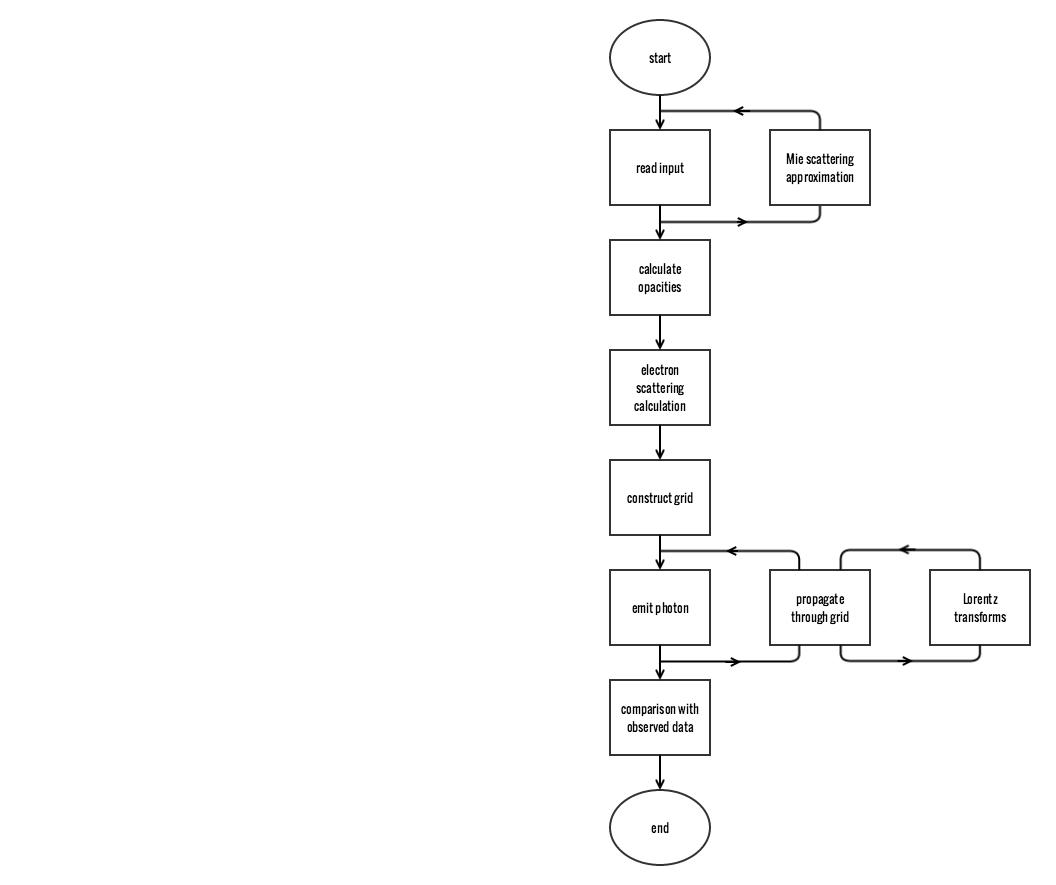
\includegraphics[scale=0.8, trim=200mm 0mm 0mm 0mm]{chapters/chapter2/code_flowchart.png}}
	\end{centering}
	\clearpage

		\subsubsection{Common}
		\subsubsection{Input}
		\subsubsection{Electron Scattering}
		\subsubsection{Random Routines}
		\subsubsection{Functions}
		\subsubsection{Sizes}
		\subsubsection{Global}
		\subsubsection{Photon}
		\subsubsection{Iterate}
		\subsubsection{Construct Grid}
		\subsubsection{Linear Interpolation}
		\subsubsection{Code}
		\subsubsection{Damocles}
		
	\subsection{Input}
	\subsection{Output}
	\subsection{Post-Processing and Visualisation}
\section{Limitations and Further Developments}
\label{limitations}

\clearpage
		


THE REST FOLLOW HERE. 


